% !TEX program = xelatex
% 教案例子：2D DDPM 动手实验（双月数据）
\documentclass[a4paper,fontset=none,zihao=5]{ctexart}

\setCJKmainfont{NotoSerifCJKsc-Regular}[BoldFont=NotoSerifCJKsc-Bold, ItalicFont={AR PL KaitiM GB}]
\setCJKsansfont{NotoSansCJKsc-Regular}[BoldFont=NotoSansCJKsc-Bold]
\setCJKmonofont{NotoSansMonoCJKsc-Regular}
\setmonofont{DejaVu Sans Mono}[Scale=0.93]

\usepackage[margin=1.8cm,top=2.0cm,bottom=2.0cm]{geometry}
\usepackage{amsmath,amssymb,mathtools,bm}
\usepackage{graphicx,float,caption,booktabs,enumitem,array,tabularx,longtable}
\usepackage{xcolor}
\usepackage[most]{tcolorbox}
\usepackage{listings}
\usepackage{fancyhdr}
\usepackage[unicode]{hyperref}
\usepackage{xurl}

\definecolor{ctitle}{HTML}{1E3A8A}
\definecolor{chead}{HTML}{1E40AF}
\definecolor{csub}{HTML}{334155}
\definecolor{cbox}{HTML}{EFF6FF}
\definecolor{cboxb}{HTML}{93C5FD}
\definecolor{cnote}{HTML}{9A3412}
\definecolor{cnotebg}{HTML}{FFF7ED}
\definecolor{cmuted}{HTML}{64748B}
\definecolor{cwhy}{HTML}{047857}
\definecolor{cwhybg}{HTML}{ECFDF5}
\definecolor{clink}{HTML}{1D4ED8}
\definecolor{ccodebg}{HTML}{F8FAFC}
\definecolor{ccomment}{HTML}{15803D}
\definecolor{ckw}{HTML}{7C3AED}
\definecolor{cstr}{HTML}{B45309}

\hypersetup{colorlinks=true,linkcolor=chead,urlcolor=clink,citecolor=chead,
  pdftitle={教案例子：2D DDPM 动手实验（双月数据）},pdfauthor={Grok Bot 教学笔记}}

\ctexset{
  section = {format=\Large\sffamily\bfseries\color{chead}, name={,}, number=\chinese{section}、, aftername={}, beforeskip=1.1em, afterskip=0.6em},
  subsection = {format=\large\sffamily\bfseries\color{csub}, beforeskip=0.8em, afterskip=0.4em},
}
\pagestyle{fancy}\fancyhf{}
\renewcommand{\headrulewidth}{0.4pt}
\renewcommand{\headrule}{\color{black!15}\hrule height\headrulewidth}
\fancyfoot[C]{\footnotesize\color{cmuted}2D DDPM 动手实验 · 教案例子\quad·\quad 第 \thepage{} 页}
\fancypagestyle{plain}{\fancyhf{}\renewcommand{\headrulewidth}{0pt}%
  \fancyfoot[C]{\footnotesize\color{cmuted}2D DDPM 动手实验 · 教案例子\quad·\quad 第 \thepage{} 页}}
\captionsetup{font={small,color=cmuted},labelsep=quad}
\captionsetup[figure]{name=图}
\captionsetup[table]{name=表}

\newtcolorbox{notebox}[1][]{enhanced,breakable,colback=cnotebg,colframe=cnote!45,boxrule=0.5pt,arc=2pt,
  left=6pt,right=6pt,top=4pt,bottom=4pt,fontupper=\small\color{cnote},#1}
\newtcolorbox{keybox}[1][]{enhanced,colback=cbox,colframe=cboxb,boxrule=0.6pt,arc=2pt,left=6pt,right=6pt,top=2pt,bottom=2pt,#1}
\newtcolorbox{whybox}[1][]{enhanced,breakable,colback=cwhybg,colframe=cwhy!55,boxrule=0.5pt,arc=2pt,
  left=6pt,right=6pt,top=3pt,bottom=4pt,fontupper=\small,
  title={\sffamily\bfseries 为什么这样做？},coltitle=cwhy,colbacktitle=cwhybg,attach title to upper={\quad},#1}
\newtcolorbox{stepbox}[2][]{enhanced,breakable,colback=white,colframe=chead!60,boxrule=0.6pt,arc=2pt,
  left=6pt,right=6pt,top=3pt,bottom=4pt,title={\sffamily\bfseries #2},colbacktitle=chead!8,coltitle=chead,#1}

\lstdefinestyle{py}{language=Python,basicstyle=\ttfamily\footnotesize,
  backgroundcolor=\color{ccodebg},frame=single,rulecolor=\color{black!15},
  numbers=left,numberstyle=\tiny\color{cmuted},numbersep=6pt,xleftmargin=1.6em,framexleftmargin=1.4em,
  keywordstyle=\color{ckw}\bfseries,commentstyle=\color{ccomment},stringstyle=\color{cstr},
  showstringspaces=false,breaklines=true,columns=fullflexible,keepspaces=true,tabsize=4,
  upquote=true}
\lstdefinestyle{sh}{basicstyle=\ttfamily\footnotesize,backgroundcolor=\color{ccodebg},frame=single,
  rulecolor=\color{black!15},columns=fullflexible,keepspaces=true,breaklines=true,showstringspaces=false}

\newcommand{\x}{\mathbf{x}}
\newcommand{\I}{\mathbf{I}}
\newcommand{\N}{\mathcal{N}}
\newcommand{\abar}{\bar{\alpha}}
\newcommand{\eps}{\boldsymbol{\epsilon}}
\newcommand{\epst}{\boldsymbol{\epsilon}_\theta}
\newcommand{\E}{\mathbb{E}}
\newcommand{\code}[1]{\texttt{#1}}
\newcommand{\notes}{《扩散生成模型的数学原理》讲义}

\setlength{\parskip}{0.3em}
\setlength{\emergencystretch}{3em}
\linespread{1.22}

\begin{document}
\thispagestyle{plain}
\begin{center}
  \vspace*{0.6cm}
  {\sffamily\bfseries\fontsize{22}{30}\selectfont\color{ctitle} 教案例子：亲手训练一个 2D 扩散模型\par}
  \vspace{0.4em}
  {\large\color{csub} 双月数据（make\_moons）\enspace·\enspace 小 MLP 预测噪声\enspace·\enspace CPU 约 20 秒出结果\par}
  \vspace{0.4em}
  {\color{chead}\rule{0.6\textwidth}{1.5pt}\par}
  \vspace{0.2em}
  {\small\color{cmuted} 配套讲义：\notes（\code{diffusion\_math\_teaching\_notes\_latex.pdf}）\par}
\end{center}

\begin{keybox}
\small
\renewcommand{\arraystretch}{1.25}
\begin{tabularx}{\linewidth}{@{}>{\bfseries}p{0.15\linewidth}X@{}}
课题 & DDPM 的前向加噪、$\eps$ 预测训练与逐步去噪采样（2D 可视化实验） \\
对象 & 本科高年级 / 研究生；已学或正在学配套讲义第二、四章 \\
先修 & Python、PyTorch 基础（张量、\code{nn.Module}、优化器）；高斯分布与条件概率 \\
时长 & 90–120 分钟（概念 15 + 前向演示 20 + 训练采样 40 + 讨论 15–20，余量用于排错） \\
硬件 & 普通笔记本 CPU 即可，无需 GPU；数据由 sklearn 内置生成，免下载 \\
产出 & 每位学生得到：前向加噪图、loss 曲线、反向轨迹逐帧图、「数据 vs 生成」对比图 \\
\end{tabularx}
\end{keybox}

\section{教学目标}
完成本节课后，学生能够：
\begin{enumerate}[leftmargin=2em,itemsep=1pt]
  \item \textbf{前向加噪：}用闭式 $\x_t=\sqrt{\abar_t}\x_0+\sqrt{1-\abar_t}\eps$ 解释数据如何逐步变成近似高斯噪声，并在代码中一行实现；
  \item \textbf{训练目标：}说清网络 $\epst(\x_t,t)$ 预测的是\emph{加进去的噪声} $\eps$，而不是直接输出样本；写出 $\|\eps-\epst\|^2$ 损失；
  \item \textbf{反向采样：}从 $\x_T\sim\N(\mathbf 0,\I)$ 出发逐步去噪，生成双月分布，并读懂每一行采样代码对应的公式；
  \item \textbf{实验探究：}改变训练步数、$T$、$\beta$ 日程，观察对生成质量的影响，并与讲义 §3.2「小步长 $\Rightarrow$ 反向一步近似高斯」相联系。
\end{enumerate}

\begin{whybox}
\textbf{为什么选 2D 双月而不是图像？}(1) 每个样本只是平面上一个点，整个分布一张散点图就能看全，前向「糊掉」和反向「长出来」的过程一目了然；
(2) 数据由 \href{https://scikit-learn.org/stable/modules/generated/sklearn.datasets.make_moons.html}{\code{sklearn.datasets.make\_moons}} 一行生成，免下载、可复现；
(3) 网络只是几层 MLP，CPU 上几十秒就能训完，课堂成功率高；(4) 双月是\emph{多峰、非高斯}的分布，正好检验「从单峰高斯噪声生成多峰数据」这一核心能力。
\end{whybox}

\section{教学准备：材料与环境}
\subsection{文件清单（随本 PDF 打包于 \code{lab\_2d\_ddpm.zip}）}
\begin{center}\small
\begin{tabular}{@{}ll@{}}
\toprule
文件 & 用途 \\
\midrule
\code{requirements.txt} & 依赖：\code{torch>=2.0, numpy, matplotlib, scikit-learn} \\
\code{forward\_demo.py} & 环节 B：前向加噪可视化（不训练，约 2 秒） \\
\code{classroom\_ddpm.py} & 环节 C：课堂精简版（75 行，可投影 / 现场敲），见第五节 \\
\code{mean\_collapse\_demo.py} & 均值塌缩消融：MSE 回归 vs DDPM（图~\ref{fig:collapse}） \\
\code{train\_2d\_ddpm.py} & 完整版：命令行参数、余弦学习率、保存 ckpt 与 4 张图 \\
\code{runs/*/} & 本教案实测产出的图与 loss 记录（\code{losses.npy}） \\
\code{figs/} & 对比实验汇总图（训练步数 / $T$ / $\beta$） \\
\bottomrule
\end{tabular}
\end{center}

\subsection{环境安装（课前完成）}
CPU 版 PyTorch 的安装命令请按官方向导选择（OS / pip / CPU）：\url{https://pytorch.org/get-started/locally/}。Linux 下示例：
\begin{lstlisting}[style=sh]
python -m venv venv && source venv/bin/activate        # Windows: venv\Scripts\activate
pip install torch --index-url https://download.pytorch.org/whl/cpu
pip install numpy matplotlib scikit-learn
python -c "import torch, sklearn; print(torch.__version__, sklearn.__version__)"
\end{lstlisting}
本教案实测环境：Linux、8 核 CPU、Python 3.13、PyTorch 2.14.1 (CPU)、scikit-learn 1.9.1。

\subsection{运行命令}
\begin{lstlisting}[style=sh]
cd lab_2d_ddpm
python forward_demo.py                                      # 环节 B：生成 forward_demo.png
python classroom_ddpm.py                                    # 环节 C（精简版）：classroom_result.png
python train_2d_ddpm.py --T 100 --device cpu                # 完整版，默认 400 epochs
python train_2d_ddpm.py --epochs 40 --T 100 --device cpu --out runs/moons_e40   # 对照：训练太少
\end{lstlisting}

\begin{notebox}
\textbf{实测记录（本机，未经挑选，均为单次运行）。}
\begin{itemize}[leftmargin=1.4em,itemsep=0pt]
  \item \code{forward\_demo.py}：总耗时约 2.0 s。
  \item \code{train\_2d\_ddpm.py --epochs 40 --T 100}：训练 2.6 s（1240 步），最终 loss（最后 50 步均值）$=0.6824$；\textbf{生成结果仍是一团，看不出双月}（图~\ref{fig:epochs} 左）。
  \item \code{train\_2d\_ddpm.py --epochs 400 --T 100}：训练 22.1 s（12400 步，含采样作图共 24.7 s），最终 loss $=0.6095$；生成清晰双月（图~\ref{fig:gen}）。
  \item \code{classroom\_ddpm.py}（400 轮，无学习率衰减）：总耗时 24.7 s，末批 loss $=0.622$，生成双月（图~\ref{fig:classroom}）。
\end{itemize}
因此原方案中的 \code{--epochs 40} 只够看到 loss 下降，\textbf{不足以生成双月}；脚本默认值已改为 400（见第十节「脚本修订记录」）。
\end{notebox}

\section{课堂流程（90–120 分钟）}

\begin{stepbox}{环节 A｜概念导入（15 分钟）}
\textbf{教师活动：}在黑板画三格示意：「数据 $\to$ 噪声」（前向，固定）、「噪声 $\to$ 数据」（反向，要学）、「网络学什么」。写出第四节板书第 (1) 行，
强调训练时\emph{不需要}逐步加噪（闭式一步到位）。展示讲义图 0 / 图 4（总览与反向轨迹）。\\
\textbf{学生活动：}回答提问「如果把一张图加够多的噪声，最后还能看出原图吗？」；预测：网络的输出应该和什么同维？\\
\textbf{检查点：}学生能说出 $\x_T$ 近似 $\N(\mathbf 0,\I)$，且与 $\x_0$ 几乎无关。
\end{stepbox}

\begin{stepbox}{环节 B｜前向演示，不训练（20 分钟）}
\textbf{教师活动：}运行 \code{forward\_demo.py}，投影图~\ref{fig:forward}；指出每个子图标题里的 $\abar_t$。
引导观察：$t=20$ 时双月仍可辨，$t=50$ 已糊成一团，$t=99$ 接近各向同性高斯。\\
\textbf{学生活动：}修改 \code{ts = [0, 20, 50, 99]} 为其他时刻；把 \code{beta1} 改成 \code{0.05} 再运行，比较 $\abar_{99}$。\\
\textbf{检查点：}学生能解释 $\sqrt{\abar_t}$ 是「信号剩多少」，$\sqrt{1-\abar_t}$ 是「噪声有多大」；并注意到 $T=100$ 时 $\abar_{T}\approx0.36$（并非严格的纯噪声，留到讨论环节）。
\end{stepbox}

\begin{stepbox}{环节 C｜训练与采样（40 分钟）}
\textbf{教师活动：}逐段讲解第五节代码（日程 $\to$ 网络 $\to$ 数据 $\to$ 训练 $\to$ 采样），对照表~\ref{tab:map} 指出每个公式落在哪一行。
先让大家跑 \code{--epochs 40}（约 3 秒）：loss 在降，但生成是一团——引出「loss 下降 $\neq$ 生成好」；再跑默认 400 轮（约 25 秒）。\\
\textbf{学生活动：}运行 \code{classroom\_ddpm.py} 或完整版；记录 loss；观察 \code{reverse\_frames.png} 的逐帧演化；在代码第 64 行旁用注释写出对应公式。\\
\textbf{检查点：}得到双月形状的生成点云（允许毛边与少量「桥」）；能指出第 50 行就是重参数化闭式。
\end{stepbox}

\begin{stepbox}{环节 D｜讨论与布置作业（15–20 分钟）}
\textbf{教师活动：}展示第七节对比实验（训练步数、$T=20/100/200$、$\beta_{\text{end}}$），组织讨论第八节问题 1–4；布置作业。\\
\textbf{学生活动：}小组讨论并汇报；课后完成作业（换成 \code{make\_circles} 或高斯混合）。\\
\textbf{检查点：}学生能口述「网络预测的是 $\eps$」以及「为什么步子要小」。
\end{stepbox}

\section{板书三行公式}
记号同讲义：$\alpha_t=1-\beta_t$，$\abar_t=\prod_{s=1}^t\alpha_s$，$\eps,\mathbf z\sim\N(\mathbf 0,\I)$，$t\in\{1,\dots,T\}$。
\begin{keybox}
\begin{align}
  \text{(1) 前向（闭式）：}\quad & \x_t=\sqrt{\abar_t}\,\x_0+\sqrt{1-\abar_t}\,\eps, \label{eq:fwd}\\
  \text{(2) 训练：}\quad & L(\theta)=\E_{t,\x_0,\eps}\Big[\big\|\eps-\epst(\x_t,t)\big\|^2\Big], \label{eq:loss}\\
  \text{(3) 反向一步：}\quad & \x_{t-1}=\frac{1}{\sqrt{\alpha_t}}\Big(\x_t-\frac{\beta_t}{\sqrt{1-\abar_t}}\,\epst(\x_t,t)\Big)+\sigma_t\,\mathbf z,\qquad
  \sigma_t=\sqrt{\beta_t}\ (t>1),\ \ \sigma_1\mathbf z\equiv\mathbf 0 . \label{eq:rev}
\end{align}
\end{keybox}
\begin{whybox}
\textbf{为什么只需这三行？}(1) 让训练时对任意 $t$ 一步构造 $\x_t$（讲义 §2.3–2.4）；(2) 是 ELBO 去权重后的简化损失（讲义式 (4.9)）；
(3) 中括号部分是用网络噪声表达的反向均值 $\boldsymbol\mu_\theta$（讲义式 (3.43)），再加上方差 $\sigma_t^2$ 的高斯噪声——小步长下反向一步近似高斯（讲义 §3.2）。
最后一步（$t=1$）不加噪声：此时均值就是对干净数据的最终估计。
\end{whybox}

\section{核心代码（课堂精简版，带中文注释）}
下列代码即 \code{classroom\_ddpm.py} 全文（行号与表~\ref{tab:map} 对应）。\textbf{下标约定：}代码数组从 0 开始，\code{betas[i]} 对应公式中的 $\beta_{i+1}$；
因此代码的 \code{i == 0} 就是公式里的最后一步 $t=1$。
\lstinputlisting[style=py]{classroom_ddpm.py}

\subsection{公式 \texorpdfstring{$\leftrightarrow$}{<->} 代码对照表}
\begin{table}[!htbp]
\centering\small
\renewcommand{\arraystretch}{1.3}
\caption{板书公式与 \code{classroom\_ddpm.py} 代码行对照}
\label{tab:map}
\begin{tabularx}{\linewidth}{@{}p{0.31\linewidth}>{\raggedright\arraybackslash}p{0.10\linewidth}X@{}}
\toprule
公式 & 行号 & 代码 / 说明 \\
\midrule
$\beta_t$ 线性日程，$\alpha_t=1-\beta_t$ & 10–11 & \code{betas = torch.linspace(1e-4, 2e-2, T)}；\code{alphas = 1 - betas} \\
$\abar_t=\prod_{s\le t}\alpha_s$ & 12 & \code{torch.cumprod(alphas, 0)}：累乘 \\
$\sqrt{\abar_t},\ \sqrt{1-\abar_t}$ & 13 & 预先算好，训练时按 \code{t} 索引 \\
$t\sim\mathrm{Uniform}\{1..T\}$ & 48 & \code{torch.randint(0, T, ...)}：每个样本独立抽 $t$（代码下标 0..T-1） \\
$\eps\sim\N(\mathbf 0,\I)$ & 49 & \code{torch.randn\_like(xb)}：每次新抽，\emph{不可复用} \\
式 \eqref{eq:fwd}：$\x_t=\sqrt{\abar_t}\x_0+\sqrt{1-\abar_t}\eps$ & 50 & \code{sa[t].unsqueeze(1) * xb + sm[t].unsqueeze(1) * eps}；\code{unsqueeze(1)} 把 $(B,)$ 广播到 $(B,2)$ \\
$\epst(\x_t,t)$ & 16–35 & 正弦时间嵌入 + 4 层 MLP；输出维度 2 = 数据维度 \\
式 \eqref{eq:loss}：$\|\eps-\epst\|^2$ & 51 & \code{mse\_loss(net(xt, t), eps)}（对维度与批取平均，差常数倍） \\
$\x_T\sim\N(\mathbf 0,\I)$ & 59 & \code{torch.randn(n, 2)} \\
$t=T,\dots,1$ & 60 & \code{for i in reversed(range(T))}：\code{i}$=t-1$ \\
式 \eqref{eq:rev} 中的 $\boldsymbol\mu_\theta$ & 62–64 & \code{(x - beta/sqrt(1-ab)*eps) / sqrt(alpha)} \\
$+\sigma_t\mathbf z,\ \sigma_t=\sqrt{\beta_t}$ & 66 & \code{mean + torch.sqrt(beta) * torch.randn\_like(x)} \\
$t=1$ 不加噪声 & 67–68 & \code{i == 0} 时 \code{x = mean} \\
\bottomrule
\end{tabularx}
\end{table}

\begin{whybox}
\textbf{为什么时间 $t$ 要做正弦嵌入再拼接？}同一个网络要处理所有噪声水平：$t$ 小时只需微调，$t$ 大时要「猜」出大部分噪声。
直接输入整数 $t$ 尺度过大且难以表达；正弦 / 余弦多频率嵌入（与 Transformer 位置编码同源）给网络一组平滑、可区分的时间特征。
\textbf{为什么数据要标准化？}前向过程是「方差保持」的（讲义 §2.1），只有数据本身方差约为 1，$\x_T$ 才接近 $\N(\mathbf 0,\I)$，采样起点才与训练一致。
\end{whybox}

\section{预期结果（实测图）}
\begin{figure}[H]
  \centering
  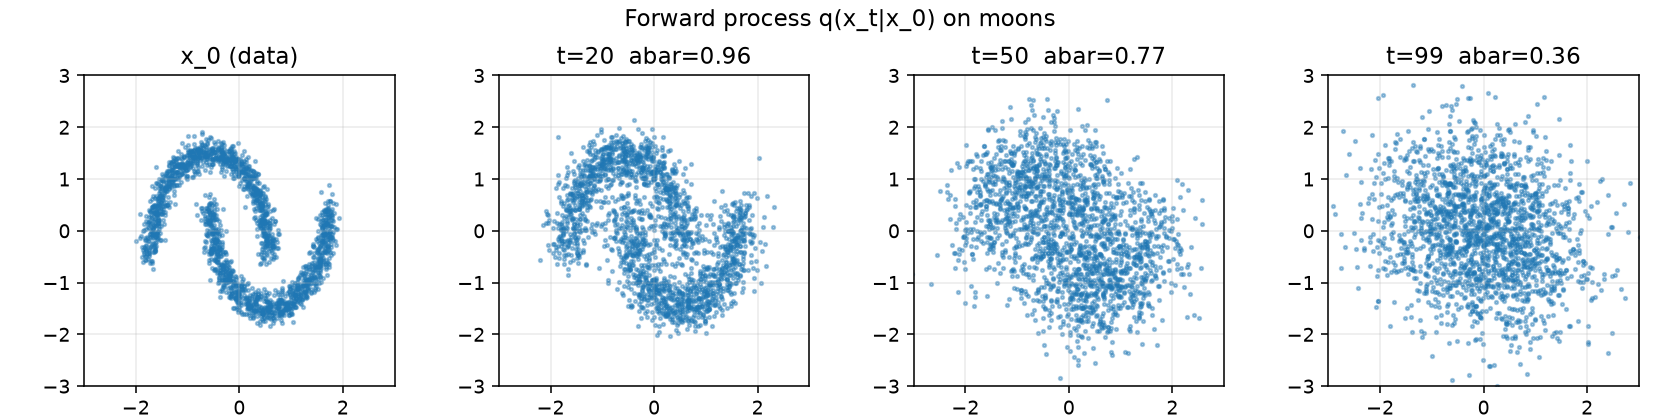
\includegraphics[width=\textwidth]{forward_demo.png}
  \caption{环节 B：\code{forward\_demo.py} 实测输出。标题中的 abar 即 $\abar_t$（代码下标）。$t=99$ 时 $\abar\approx0.36$，点云已近似各向同性高斯。}
  \label{fig:forward}
\end{figure}

\begin{figure}[H]
  \centering
  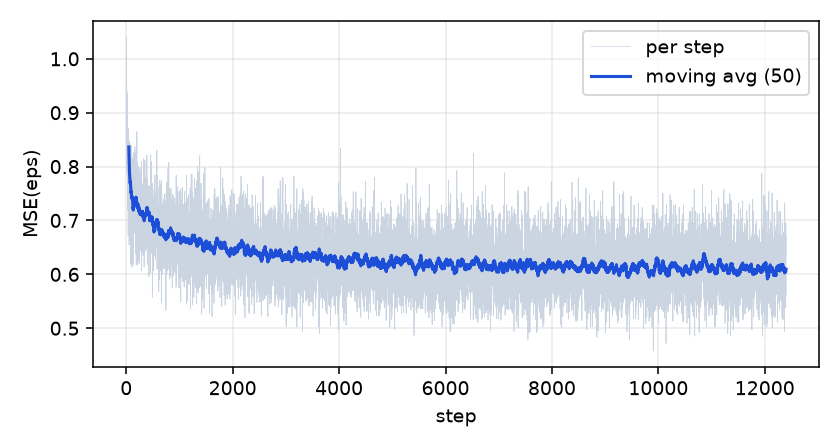
\includegraphics[width=0.62\textwidth]{runs/moons_e400/loss.png}
  \caption{\code{train\_2d\_ddpm.py}（400 epochs，$T=100$）的训练 loss：灰线为每步 MSE，蓝线为 50 步滑动平均。
  loss 很快降到约 0.6 后趋平——它\emph{不会}降到 0，因为小 $t$ 时噪声几乎不可辨认（见第八节问题 2）。}
  \label{fig:loss}
\end{figure}

\begin{figure}[H]
  \centering
  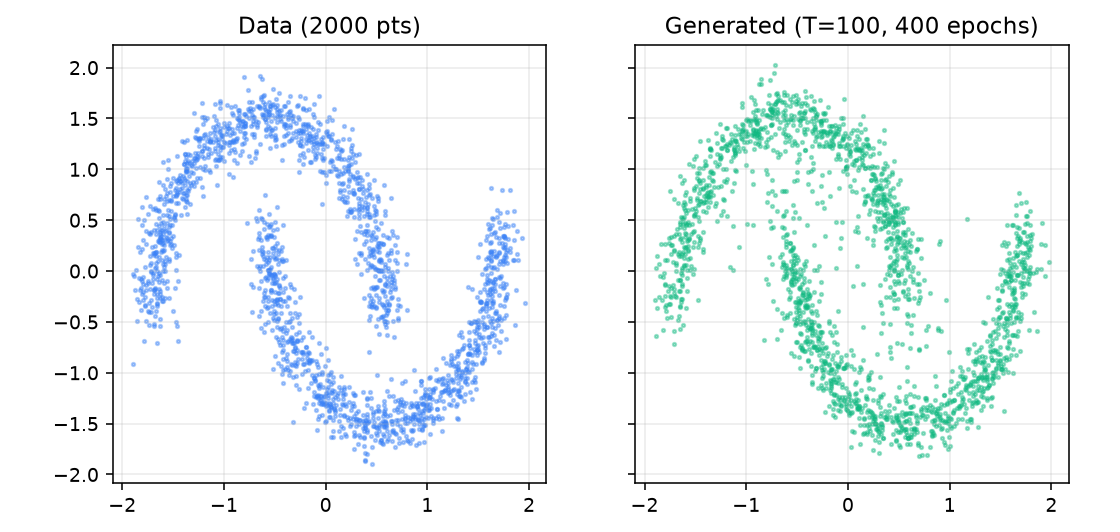
\includegraphics[width=0.66\textwidth]{runs/moons_e400/data_vs_generated.png}
  \caption{左：训练数据（2000 点）；右：模型从纯噪声生成的 2000 个点（400 epochs，$T=100$）。}
  \label{fig:gen}
\end{figure}

\begin{figure}[H]
  \centering
  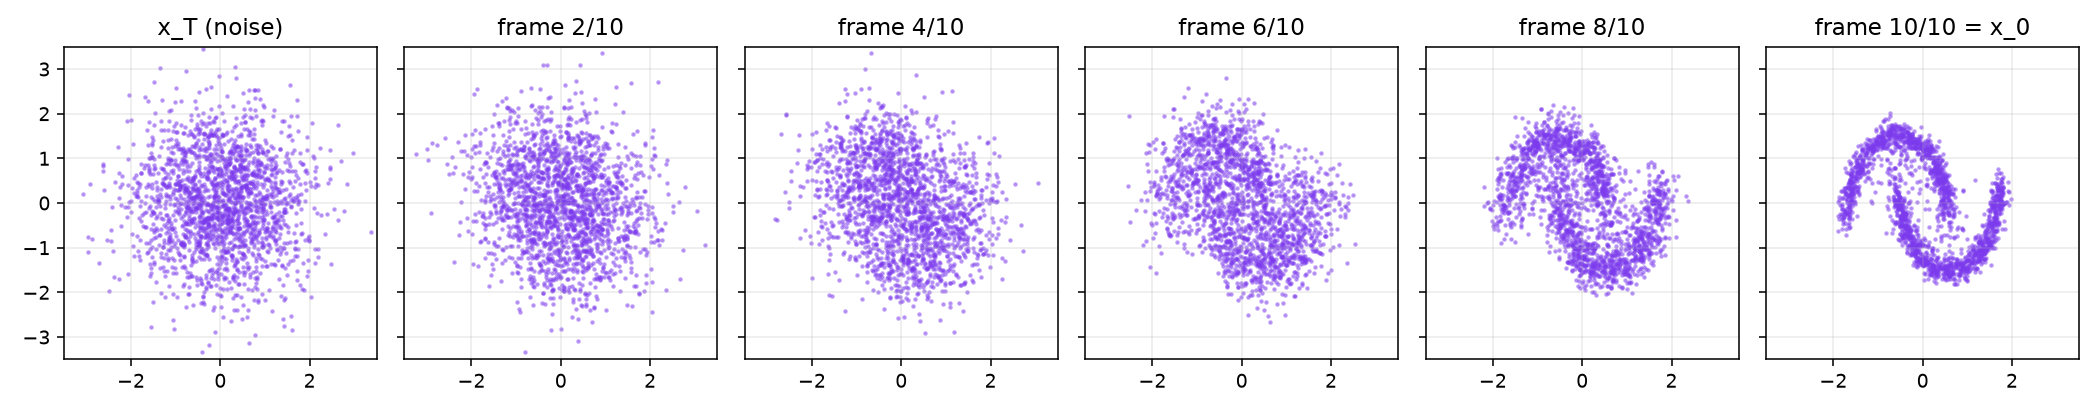
\includegraphics[width=\textwidth]{runs/moons_e400/reverse_frames.png}
  \caption{反向采样轨迹逐帧图（每 10 步记录一帧）：噪声团 $\to$ 模糊月牙 $\to$ 清晰双月。}
  \label{fig:frames}
\end{figure}

\begin{figure}[H]
  \centering
  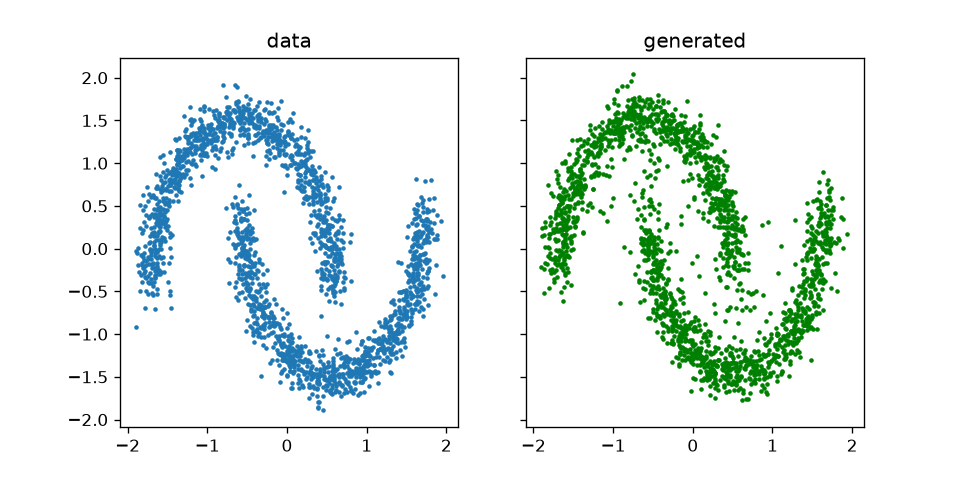
\includegraphics[width=0.6\textwidth]{classroom_result.png}
  \caption{课堂精简版 \code{classroom\_ddpm.py} 的实测输出（400 轮，约 25 s）。}
  \label{fig:classroom}
\end{figure}


\section{为什么不能用「普通回归」生成双月？}
扩散模型的训练损失也是 MSE，看起来很像「回归」。那为什么不直接训练一个网络预测 $x_0$，在 $t=T$ 时喂进噪声、一次输出 $\hat x_0$ 当样本？答案是：\textbf{MSE 最优解是条件均值 $E[x_0|x_t]$，多峰分布下均值落在峰与峰之间}。

\begin{whybox}
\textbf{均值塌缩（mean collapse）。}双月是双峰分布。当噪声很大（$t$ 接近 $T$）时，一个噪声点 $\x_t$ 几乎同样可能来自左月或右月，于是
\[
  E[\x_0\mid\x_t]\ \approx\ \tfrac12\,\x_{\text{左}}+\tfrac12\,\x_{\text{右}}
\]
落在两月\emph{之间}的空隙——数据支撑集上概率几乎为 0 的地方。网络若用 MSE 回归 $\x_t\to\x_0$，学到的正是这个均值；一次去噪得到的「样本」就会堆成原点附近的一团，而不是两条月牙。\\
DDPM 不输出这个均值当样本，而是学习噪声 / score，再通过\emph{多步随机}反向过程从 $p(\x_0\mid\x_t)$ 里抽样——每一步只走一小步，并加上噪声，才能分别落到左月或右月。
\end{whybox}

实测消融（脚本 \code{mean\_collapse\_demo.py}；$\x_0$-回归器与 DDPM 使用同容量 MLP，$T=100$）：
\begin{figure}[H]
  \centering
  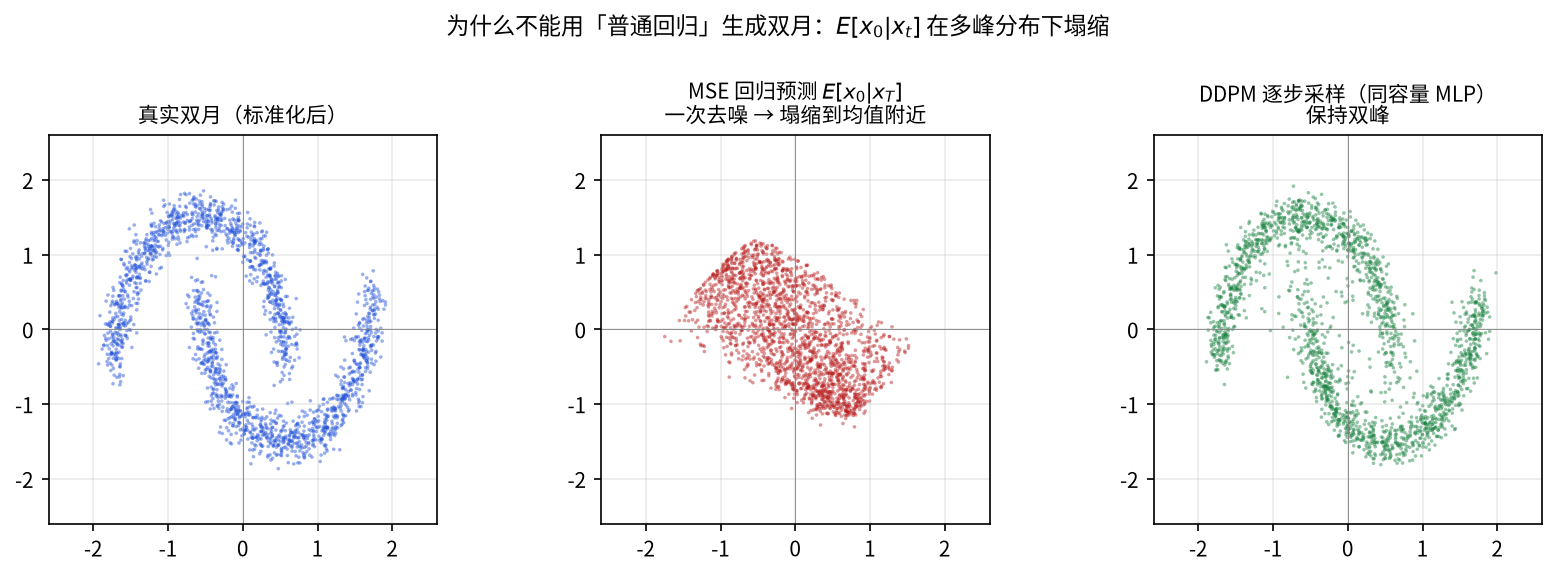
\includegraphics[width=\textwidth]{figs/mean_collapse.png}
  \caption{左：真实双月；中：从 $\x_T\sim\N(\mathbf 0,\I)$ 一次回归 $\hat\x_0=E[\x_0|\x_T]$（塌缩，均值约 $(-0.02,-0.07)$，std $\approx0.62$）；右：同容量 DDPM 逐步采样（保持双峰，std $\approx1.0$）。}
  \label{fig:collapse}
\end{figure}
\begin{figure}[H]
  \centering
  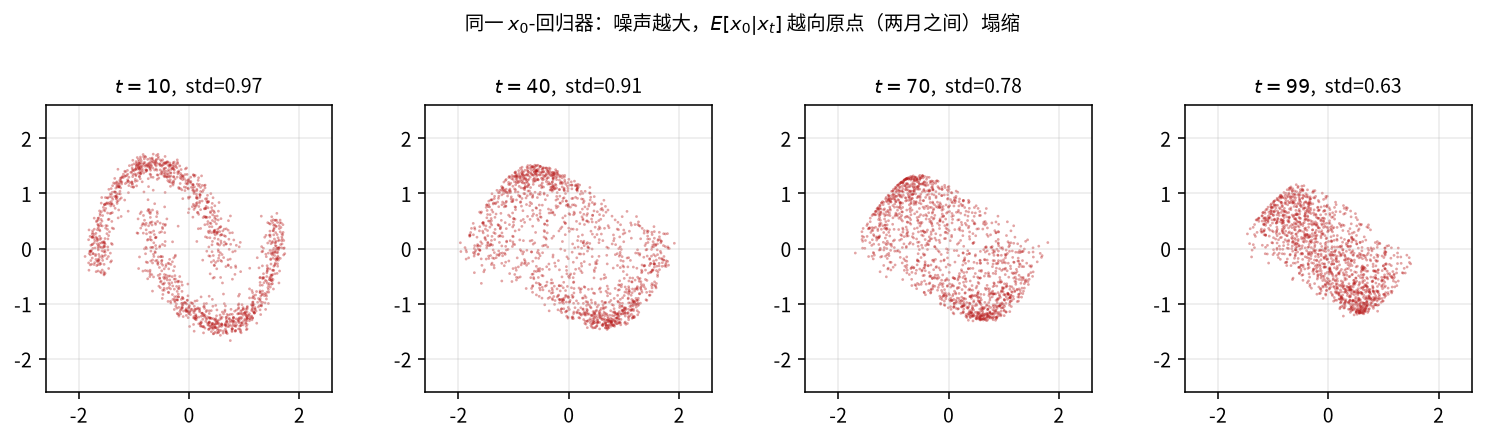
\includegraphics[width=\textwidth]{figs/mean_collapse_by_t.png}
  \caption{同一 $\x_0$-回归器在不同 $t$ 上的预测：小 $t$ 仍见双月，随噪声增大逐渐并成一团（std：$0.97\to0.91\to0.78\to0.63$）。}
  \label{fig:collapse-t}
\end{figure}

\begin{notebox}
\textbf{与板书公式的关系。}训练时写的是 $\E\|\eps-\epst(\x_t,t)\|^2$，其最优解等价于预测 $E[\eps|\x_t]$（或等价的 $E[\x_0|\x_t]$）。损失学到的是均值，\emph{生成}靠的是采样过程——这正是「知其然又知其所以然」：MSE 负责拟合后验均值 / score，祖先采样负责从后验里抽一个样本，而不是把均值当成样本。
\end{notebox}

\section{验收清单与对比实验}
\subsection{验收（「看到效果」）}
\begin{itemize}[leftmargin=1.6em,itemsep=1pt]
  \item[$\square$] loss 曲线总体下降并趋平（图~\ref{fig:loss}）；
  \item[$\square$] 生成点云呈双月形状（允许毛边和少量连接两月的「桥」，图~\ref{fig:gen}）；
  \item[$\square$] 反向轨迹呈现「噪声团 $\to$ 模糊月牙 $\to$ 清晰双月」（图~\ref{fig:frames}）；
  \item[$\square$] 能口述：网络预测的是噪声 $\eps$，不是直接输出样本；能指出代码中三行板书公式的位置。
\end{itemize}

\subsection{对比实验（实测，均为单次运行）}
\begin{figure}[H]
  \centering
  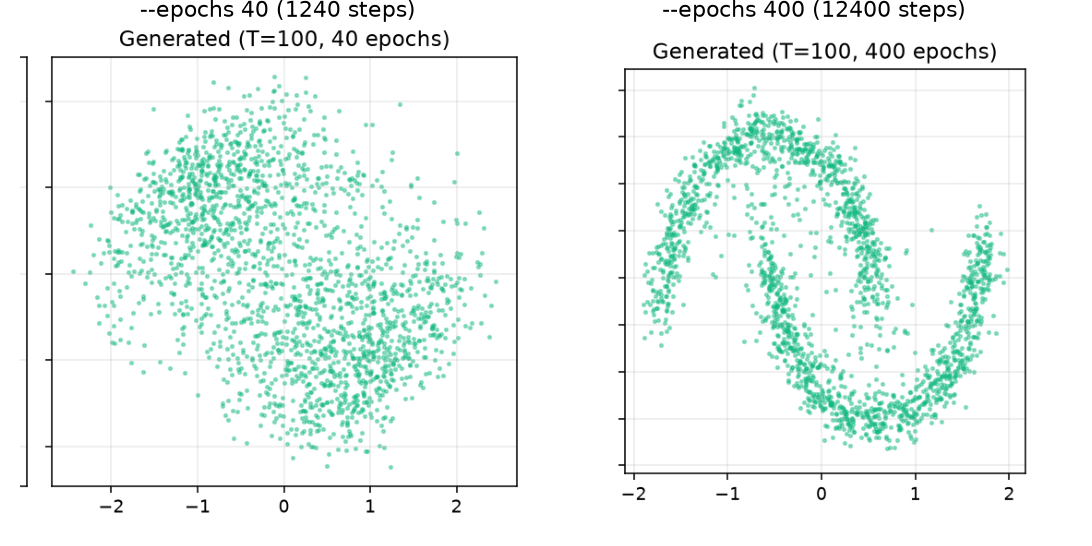
\includegraphics[width=0.62\textwidth]{figs/cmp_epochs.png}
  \caption{训练步数的影响（$T=100$）：40 epochs（1240 步，loss 0.6824）只得到一团；400 epochs（12400 步，loss 0.6095）得到双月。}
  \label{fig:epochs}
\end{figure}
\begin{figure}[H]
  \centering
  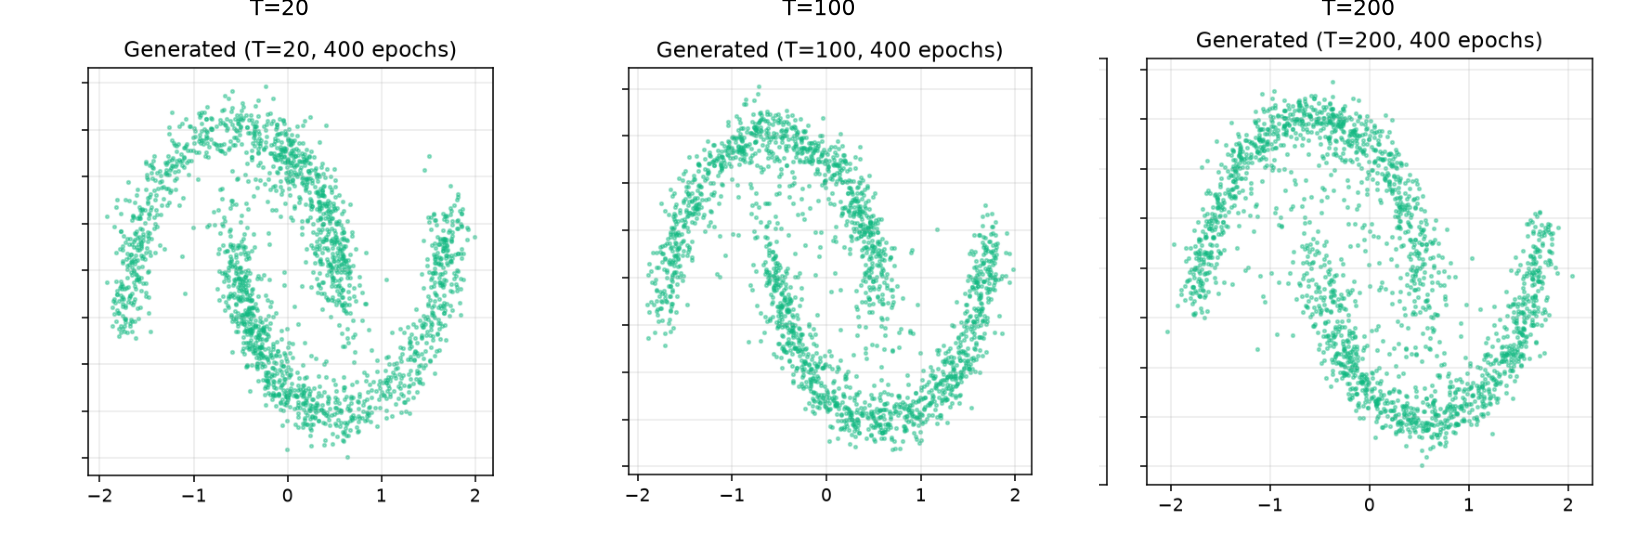
\includegraphics[width=0.9\textwidth]{figs/cmp_T.png}
  \caption{$T=20/100/200$（$\beta$ 均为 $10^{-4}\to0.02$，400 epochs）。实测训练时间 19.5 s / 22.1 s / 19.8 s；
  $\abar_T$ 分别为 0.82 / 0.36 / 0.13。三者都能生成双月，差别主要在毛边与「桥」的多少。}
  \label{fig:T}
\end{figure}
\begin{figure}[H]
  \centering
  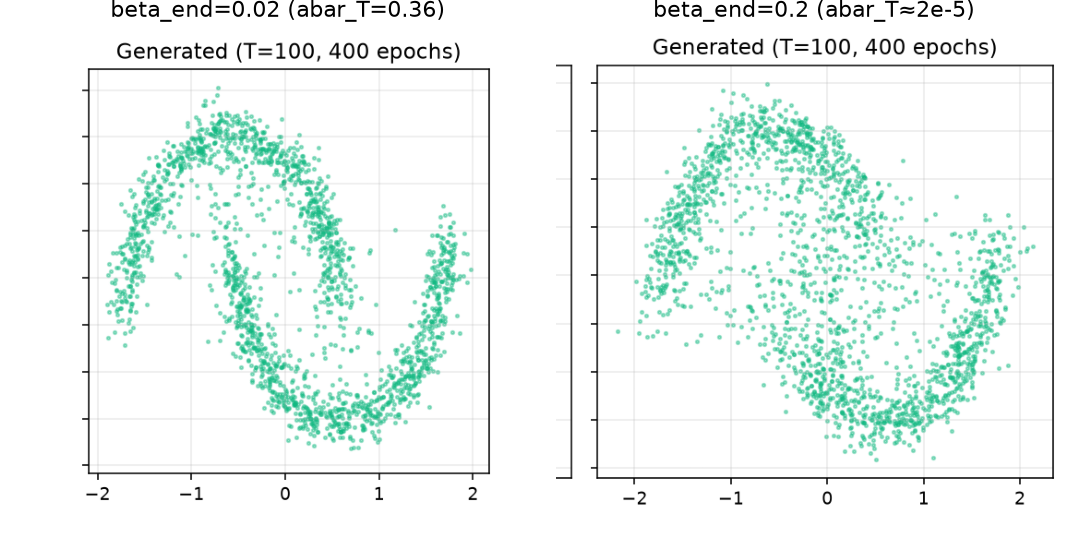
\includegraphics[width=0.62\textwidth]{figs/cmp_beta.png}
  \caption{$\beta_{\text{end}}=0.02$ 与 $0.2$（$T=100$，400 epochs）。后者 $\abar_T\approx2\times10^{-5}$（起点更像纯噪声），但每步 $\beta_t$ 大 10 倍，生成的月牙之间「桥」明显更多。}
  \label{fig:beta}
\end{figure}

\begin{notebox}
\textbf{注意：}不同日程下 loss 数值不可直接比较（$\beta_{\text{end}}=0.2$ 时 loss 仅 0.243，但生成更差）——因为 $t$ 的分布中「容易猜噪声」的高噪声时刻占比不同。
以生成图而不是 loss 数值评价质量。
\end{notebox}

\section{讨论问题与作业}
\subsection{课堂讨论}
\begin{enumerate}[leftmargin=2em,itemsep=2pt]
  \item 为什么 MSE 回归 $\x_t\to\x_0$ 会得到两月之间的一团，而 DDPM 不会？（提示：最优解是 $E[\x_0|\x_t]$，生成靠采样。）
  \item \textbf{loss 在降，生成却是一团（图~\ref{fig:epochs}）。为什么？}提示：loss 是对所有 $t$ 的平均；大 $t$ 的噪声很好猜，小 $t$ 的精细结构需要更多训练步才学得会。
  \item \textbf{为什么 loss 不会降到 0？}提示：给定 $\x_t$，$\eps$ 并不唯一确定（不同 $\x_0$ 都可能产生同一 $\x_t$）；最优网络输出的是条件期望 $\E[\eps\mid\x_t]$（讲义 §4.1 为什么框、§3.2 第 5 步）。
  \item \textbf{$T=100$ 时 $\abar_T\approx0.36$，但我们从 $\N(\mathbf 0,\I)$ 出发也能生成，为什么？把 $\beta$ 放大到 0.2 让 $\abar_T\approx0$ 反而更差（图~\ref{fig:beta}），又为什么？}
        提示：数据已标准化，$\x_T$ 的边缘方差恰为 1、形状已接近高斯；而大 $\beta_t$ 让反向一步不再近似高斯（讲义 §3.2 第 4 步、图 5）。这是「起点误差」与「每步高斯近似误差」之间的权衡。
  \item \textbf{采样时最后一步为什么不加噪声？若每步都不加噪声（$\sigma_t=0$）会怎样？}动手试：把第 66 行的噪声项去掉，观察样本是否塌缩到月牙的「中心线」。
\end{enumerate}

\subsection{课后作业}
\begin{enumerate}[leftmargin=2em,itemsep=2pt]
  \item \textbf{$T$ 与步长：}分别用 \code{--T 20} 与 \code{--T 200} 训练（可加 \code{--beta-end}），把三张生成图放在一起，写 150 字分析。
  \item \textbf{$\beta$ 日程：}实现讲义提到的 cosine schedule（Nichol \& Dhariwal 2021，\href{https://arxiv.org/abs/2102.09672}{arXiv:2102.09672}），与线性日程对比生成质量与 $\abar_T$。
  \item \textbf{换数据：}把 \code{make\_moons} 换成 \href{https://scikit-learn.org/stable/modules/generated/sklearn.datasets.make_circles.html}{\code{make\_circles}}，或自己写一个 8 个高斯的混合（环形排列）；观察模型能否覆盖所有模态。
  \item \textbf{采样方差：}把 $\sigma_t=\sqrt{\beta_t}$ 换成 $\sigma_t=\sqrt{\tilde\beta_t}$，$\tilde\beta_t=\frac{1-\abar_{t-1}}{1-\abar_t}\beta_t$（讲义式 (3.37)），比较结果。
\end{enumerate}

\section{常见问题与排错}
\begin{center}\small
\renewcommand{\arraystretch}{1.3}
\begin{tabularx}{\linewidth}{@{}>{\raggedright\arraybackslash}p{0.3\linewidth}X@{}}
\toprule
现象 & 原因与处理 \\
\midrule
生成是一团高斯，看不出双月 & 训练步数太少（如 \code{--epochs 40}，仅 1240 步）。用默认 400 轮，或减小 batch。 \\
生成点云整体偏移 / 尺度不对 & 忘记标准化数据，或训练与采样用了不同的 \code{betas}。两处必须用同一套日程。 \\
采样结果全是 NaN 或爆炸 & 公式中把 $\sqrt{1-\abar_t}$ 写成 $1-\abar_t$，或把 \code{sqrt(alpha)} 写成 \code{alpha}；检查第 64 行。 \\
\code{RuntimeError: shape mismatch} & \code{sa[t]} 形状是 $(B,)$，需 \code{.unsqueeze(1)} 变成 $(B,1)$ 再与 $(B,2)$ 相乘。 \\
loss 不降 & 损失目标写成了 \code{xb} 而不是 \code{eps}；或每个 batch 复用了同一个 \code{eps}。 \\
CPU 很慢 / 多进程卡顿 & 同时跑多个训练会争抢线程；一次只跑一个，或设置 \code{torch.set\_num\_threads(4)}。 \\
最后一步多了一圈毛边 & $t=1$ 时（代码 \code{i == 0}）误加了噪声。 \\
\bottomrule
\end{tabularx}
\end{center}

\section{进阶拓展}
\begin{enumerate}[leftmargin=2em,itemsep=2pt]
  \item \textbf{MNIST + 小 U-Net：}数据见 \href{https://docs.pytorch.org/vision/stable/generated/torchvision.datasets.MNIST.html}{torchvision MNIST 文档}；有 GPU 更流畅，CPU 可减少通道数、少训几轮先看到模糊数字。
  \item \textbf{Hugging Face Diffusers：}\href{https://huggingface.co/docs/diffusers/index}{Diffusers 文档}；官方教程 \href{https://huggingface.co/docs/diffusers/tutorials/basic_training}{Train a diffusion model}（64 分辨率蝴蝶图像，可用小 batch）。
  \item \textbf{对照讲义验证「小步长」：}固定训练步数，扫描 $\beta_{\text{end}}\in\{0.01,0.02,0.05,0.1,0.2\}$ 与 $T$，画「生成质量 vs 每步 $\beta_t$」曲线，直观验证讲义 §3.2 的结论。
  \item \textbf{原论文代码：}DDPM 官方实现 \href{https://github.com/hojonathanho/diffusion}{hojonathanho/diffusion}（TensorFlow），可对照本课代码中的日程与采样公式。
\end{enumerate}

\section{与配套数学讲义的衔接}
\begin{center}\small
\renewcommand{\arraystretch}{1.3}
\begin{tabularx}{\linewidth}{@{}>{\raggedright\arraybackslash}p{0.33\linewidth}X@{}}
\toprule
本实验环节 / 代码 & 讲义对应位置 \\
\midrule
环节 B、代码第 10–13、50 行 & §2.1 前向定义（式 2.1）；§2.3 闭式（式 2.4）；§2.4 重参数化；§2.5 $\beta$ 日程 \\
代码第 51 行（损失） & §4.3 简化损失 $L_{\text{simple}}$（式 4.9）；§4.4 算法 1 \\
代码第 62–68 行（采样） & §3.5 $\boldsymbol\mu_\theta$ 的 $\eps$ 形式（式 3.43）；§5 算法 2 \\
讨论问题 3（大 $\beta$ 更差） & §3.2「为什么可以把反向一步建模为高斯」第 2–4 步与图 5 \\
讨论问题 2（loss 不为 0） & §4.1 为什么框（最优解为条件期望）；§3.2 第 5 步 \\
作业 4（$\tilde\beta_t$） & §3.3 固定方差的为什么框；§3.4 后验方差（式 3.37） \\
\bottomrule
\end{tabularx}
\end{center}
\textbf{建议顺序：}先讲讲义第二章（前向闭式）与 §4.3（$\eps$-loss）$\to$ 立即上本实验 $\to$ 回到第三章讲反向贝叶斯推导与「小步长高斯近似」，用本实验的对比图作为直观证据。

\section{脚本修订记录（相对原始方案）}
运行原方案时发现并处理了以下问题（所有数字均来自本机实测）：
\begin{enumerate}[leftmargin=2em,itemsep=2pt]
  \item \textbf{训练步数不足：}原命令 \code{--epochs 40}（$8000/256\approx31$ 步/轮，共 1240 步）生成结果是一团。\code{train\_2d\_ddpm.py} 默认改为 400 轮（约 22 s），精简版同步改为 400 轮。
  \item \textbf{缺少随机种子：}两份脚本原先结果不可复现，已加 \code{torch.manual\_seed}。
  \item \textbf{完整版新增：}余弦学习率衰减、命令行参数 \code{--beta-end}、训练计时与最终 loss 打印、额外输出 \code{data\_vs\_generated.png}、\code{reverse\_frames.png}、\code{loss.png}。
  \item \textbf{前向演示：}子图标题显示 $\abar_t$，让学生直接看到 $T=100$ 时 $\abar_T\approx0.36$。
  \item \textbf{关于 $\abar_T$ 未归零：}曾尝试按 $1000/T$ 放大 $\beta$（$\abar_T\approx2\times10^{-5}$），实测生成反而更差（图~\ref{fig:beta}），故保留原线性日程，并把它作为讨论问题 3。
\end{enumerate}

\section{参考资料与链接}
\small
\begin{enumerate}[label={[\arabic*]},leftmargin=2.2em,itemsep=2pt]
  \item J. Ho, A. Jain, P. Abbeel. Denoising Diffusion Probabilistic Models. NeurIPS 2020. \url{https://arxiv.org/abs/2006.11239}
  \item DDPM 官方代码：\url{https://github.com/hojonathanho/diffusion}
  \item Y. Song et al. Score-Based Generative Modeling through Stochastic Differential Equations. ICLR 2021. \url{https://arxiv.org/abs/2011.13456}
  \item A. Nichol, P. Dhariwal. Improved Denoising Diffusion Probabilistic Models. ICML 2021. \url{https://arxiv.org/abs/2102.09672}
  \item L. Weng. What are Diffusion Models? (blog, 2021). \url{https://lilianweng.github.io/posts/2021-07-11-diffusion-models/}
  \item PyTorch 安装向导：\url{https://pytorch.org/get-started/locally/}
  \item scikit-learn \code{make\_moons}：\url{https://scikit-learn.org/stable/modules/generated/sklearn.datasets.make_moons.html}
  \item scikit-learn \code{make\_circles}：\url{https://scikit-learn.org/stable/modules/generated/sklearn.datasets.make_circles.html}
  \item torchvision MNIST：\url{https://docs.pytorch.org/vision/stable/generated/torchvision.datasets.MNIST.html}
  \item Hugging Face Diffusers 文档：\url{https://huggingface.co/docs/diffusers/index}
  \item Diffusers 教程 Train a diffusion model：\url{https://huggingface.co/docs/diffusers/tutorials/basic_training}
\end{enumerate}
{\footnotesize\color{cmuted} 以上链接均已于 2026-10-10 逐一访问验证（HTTP 200）。}

\end{document}
